\documentclass[a4paper,11pt]{report}
 
 \usepackage[left=3cm, right=3cm, top=3cm, bottom=3cm]{geometry}
\usepackage{graphicx}
\usepackage{listings}
\usepackage{titlesec}
\usepackage{fancyhdr}
\usepackage{epstopdf}
\usepackage{float}
\usepackage{amsmath}
\usepackage{setspace}
\usepackage{eufrak}
\usepackage{url}

\usepackage{courier}
 \newcommand{\textform}[1]{\fontsize{14}{20}\selectfont{#1}}
\pagestyle{fancy}
\fancyhf{}
\fancyhead[R]{\thepage}
\renewcommand{\chaptermark}[1]{\markboth{#1}{}}
\renewcommand{\headrulewidth}{1pt}
\renewcommand{\footrulewidth}{1pt}

\lhead{\footnotesize{SELF SUPERVISED GRAPH NEURAL NETWORKS
}}
\rhead{}
\lfoot{\footnotesize{Department of Computer Science \& Engg.}}
\cfoot{}
\rfoot{\thepage}

\titleformat{\chapter}[display]
{\normalfont\Large\bfseries\centering}{\chaptertitlename\
\thechapter}{20pt}{\Large}


%\title{\textbf{A seminar report on\\TRUSTWORTHINESS MANAGEMENT IN THE SOCIAL INTERNET OF THINGS} 
%}
%\author{\textbf{Deena Jose}}

\begin{document}

\thispagestyle{empty}
  \begin{center}
      \fontsize{22}{25}\selectfont{\textbf{GOVERNMENT POLYTECHNIC COLLEGE PERUMBAVOOR}}\\[.1cm]
            \fontsize{15}{25}\selectfont{\textbf{Koovappady P.O Ernakulam-683 544 Kerala
    }}\\[1.2cm]
\begin{figure}[h]
	\centering
	\hspace{21pt}
	
\includegraphics[width=.50\linewidth]{logo.png}
\end{figure}

\fontsize{14}{25}\selectfont{\textbf{Semester - VI}}\\
\fontsize{14}{25}\selectfont{\textbf{Computer Engineering 2022-23}}\\[1.2cm]

\fontsize{14}{25}\selectfont{\textbf{A SEMINAR REPORT}}\\[.1cm]
    \fontsize{14}{25}\selectfont{on}\\
    \fontsize{20}{25}\selectfont{\textbf{SELF SUPERVISED GRAPH NEURAL NETWORKS
    }}\\[1.2cm]
    \fontsize{12}{25}\selectfont{\textbf{Submitted by}}\\[.2cm]
    \fontsize{14}{25}\selectfont \bfseries{VISHNU SURESH}\\[.1cm]
    \fontsize{12}{25}\selectfont{\textbf{20130132}}\\[.2cm]
%\vfill
 \end{center}

\fontsize{12pt}{20}\selectfont
\thispagestyle{empty}


\newpage
  \thispagestyle{empty}

    \begin{center}
      \fontsize{14}{20}\selectfont \textbf{GOVERNMENT POLYTECHNIC COLLEGE PERUMBAVOOR}\\
     
    \fontsize{14}{20}\selectfont \textbf{
DEPARTMENT OF COMPUTER ENGINEERING}\\[1.5cm]
\begin{figure}[h]
\centering
	\hspace{.5cm}

\includegraphics[width=0.3\linewidth]{logo.png}
\end{figure}

     
      \textbf{CERTIFICATE}
    \end{center}
    \vspace{.5cm}
    \textform{This is to certify that the seminar report entitled \textbf{Self Supervised Graph Neural Networks} submitted by \textbf{Vishnu Suresh} is approved for submission requirement for 6009 -Project and Seminar in  $6^{th}$ semester Computer Engineering at Govt.Polytechnic College,Perumbavoor.}\\[0.15cm]


\begin{minipage}{.40\textwidth}
    \begin{flushleft}
        \begin{center}
            \fontsize{12}{25}\selectfont{\textbf{Head of Section}}\\[1.5cm]
        \end{center}
    \end{flushleft}
\end{minipage}
\hfill
\begin{minipage}{0.40\textwidth}
    \begin{flushright}
        \begin{center}
            \fontsize{12}{25}\selectfont{\textbf{Lecturer in Charge}}\\[1.5cm]
        \end{center}
    \end{flushright}
\end{minipage}




\vspace{1cm}
\begin{flushleft}
  \fontsize{12}{20}\selectfont \textbf{Date  :}\\
  \fontsize{12}{20}\selectfont \textbf{Place :}
\end{flushleft}
\vspace{1cm}
\begin{minipage}{.4\textwidth}
    \begin{flushleft}
    \begin{center}
    
    \fontsize{14}{25}\selectfont \bfseries{Internal Examiner}\\[.1cm]
    
%\vfill
 \end{center}
    \end{flushleft}
      \end{minipage}
\begin{minipage}{0.8\textwidth}
\begin{flushright}
\begin{center}
 
%\vfill
\fontsize{14}{25}\selectfont \bfseries{External Examiner}\\[.1cm]

\end{center}
\end{flushright}
\end{minipage}
\newpage
\fontsize{12pt}{20}\selectfont
\thispagestyle{empty}
  \renewcommand\abstractname{\textform{\textbf{ACKNOWLEDGMENT}}}
    \begin{abstract}
      \vspace{2.5cm}
      
         I would like to express my sincere gratitude to all those who have contributed to the successful completion of my seminar on self-supervised graph neural networks. This opportunity has allowed me to delve into a fascinating field of study and expand my knowledge in computer engineering.

First and foremost, I extend my heartfelt appreciation to Dr. Aiju Thomas, the Principal of Government Polytechnic College Perumbavoor. I am grateful for his constant support, guidance, and encouragement throughout my academic journey. His visionary leadership and commitment to excellence have created an environment conducive to learning and exploration.

I am indebted to Mr. Biju Peter, the Head of the Department of Computer Engineering, for his invaluable guidance and mentorship. His expertise, patience, and enthusiasm have been instrumental in shaping my understanding of the subject and honing my research skills. I am thankful for his unwavering support and valuable insights that have enriched my seminar.

I would like to extend my sincere appreciation to Mr. Glaxy George, the Lecturer in Charge of Computer Engineering. His dedication to teaching and his willingness to go the extra mile in assisting students have been invaluable. I am grateful for his guidance, constructive feedback, and inspiring lectures that have helped me develop a deeper understanding of the topic.

I would also like to acknowledge the faculty members of the Computer Engineering Department for their constant support and encouragement throughout my academic journey. Their expertise and passion for teaching have played a significant role in shaping my intellectual growth.

I would like to express my gratitude to my classmates and friends for their support and encouragement. Their presence and collaboration have made the learning experience enjoyable and memorable.

Thank you all for your unwavering support and belief in me.
    \end{abstract}
 


\thispagestyle{empty}
  \renewcommand\abstractname{\textform{\textbf{ABSTRACT}}}
    \begin{abstract}
      \vspace{1.0cm}

 \paragraph{ }Self-supervised graph neural networks refer to a class of machine learning models that can learn to extract meaningful features from graph-structured data without the need for explicit supervision. This approach involves leveraging the intrinsic structure of the graph to generate pseudo-labels or tasks that can be used to train the model.

In self-supervised graph neural networks, the model is trained on a graph dataset by predicting either the existence of edges between nodes or the labels of nodes based on their local neighborhood structure. By doing so, the model can learn to capture the underlying patterns and relationships in the graph, even in the absence of explicit supervision.

The effectiveness of self-supervised graph neural networks has been demonstrated in various applications, such as node classification, link prediction, and graph clustering. These models have the potential to enable more efficient and effective analysis of complex graph-structured data, such as social networks, biological networks, and knowledge graphs.
\end{abstract}

  \tableofcontents
\thispagestyle{empty}

\chapter{Introduction}

\paragraph{}Graph-structured data is ubiquitous in various domains, such as social networks, biological networks, and knowledge graphs. Extracting meaningful information from these complex data requires advanced machine learning techniques that can handle the inherent challenges of graph data, such as irregularity, sparsity, and high dimensionality. Graph neural networks (GNNs) have emerged as a powerful class of models that can effectively learn representations of graph-structured data.

However, traditional GNNs require explicit supervision in the form of labeled nodes or edges, which can be expensive and time-consuming to obtain. Self-supervised learning has emerged as an alternative paradigm that can alleviate the need for explicit supervision by leveraging the intrinsic structure of the data. In self-supervised learning, the model learns to perform a task that is designed to be easy to solve based on the input data. The solution to this task provides a set of pseudo-labels that can be used to train the model.

Self-supervised graph neural networks extend this concept to graph-structured data. These models are trained on unlabeled graph data by performing a self-supervised task, such as predicting the existence of edges or the labels of nodes based on their local neighborhood structure. By doing so, the model can learn to capture the underlying patterns and relationships in the graph, even in the absence of explicit supervision.

Self-supervised graph neural networks have shown promising results in various applications, such as node classification, link prediction, and graph clustering. These models have the potential to enable more efficient and effective analysis of complex graph-structured data, which can have significant implications in many fields, such as drug discovery, social network analysis, and recommendation systems.
  

  
\chapter{Downstream Tasks with Graph Data }

When talking about the downstream tasks using the graph data, we can divide them into three categories:  

\section{Node level tasks}
Tasks that are focused on nodes properties can be considered node level tasks. Node classification can be considered as an example of a node-level task. In node classification with a self-supervised learning setting, few nodes are known with their corresponding levels which we use to predict levels for nodes that are not known.
\section{Link level tasks}
Tasks that are focused on learning the representation of node pairs or properties of edges can be considered link-level tasks. Link prediction can be an example of a link-level task, where using two nodes the task is to discriminate if there is an edge between them.
\section{Graph level tasks}
Tasks that are focused on learning from multiple graphs can be considered graph-level tasks. Graph regression can be considered a graph-level task. In a self-supervised learning setting, very few amounts of graphs with their known properties can be used to infer the properties of graphs with unknown levels using an encoder trained on a few amount of graphs with known properties.

\chapter{Graph Neural Networks}

From the family of neural networks, networks that can deal with the graph representation of the data can be considered as the graph neural network. Talking about the basic computation of the graph neural network, it can consist of two main components:

\begin{itemize}
\item[•] Aggregate Operation: Aggregate information from neighbourhoods.

\item[•] Update Operation: Update node representation using the aggregated information from the aggregate operation.
\end{itemize}

Using the above components of computation, we receive and update the information in the components of a graph like a link, node, and edges. These updates can be considered as the learning part of the graph neural network. Using the GNN, we can train a network on graph-structured data. To apply this in self-supervised learning settings we are required to make some strategies, following which we can obtain good results. 

\chapter{Self Supervised Learning Strategies using graph data}

As of now, we have discussed why we should use graph data with SSL and what kind of neural network can help us with graph data. To obtain a good result from self-supervised learning with graph data, we are required to have a strong strategy to work. By looking at different works related to this field, we can divide the strategies into three categories.  

\section{Pre-training and fine-tuning}
This can be considered as a basic strategy to be followed in any self-supervised learning setting. Using this strategy, we are required to train the model in two stages. In the first stage, any encoder is trained on the predefined pretext-task, then the pre-trained parameters can be used for initializing the encoder. The second stage is the fine-tuning stage where the pre-trained encoder can be fine-tuned with a prediction head where we know about the downstream task. The below image is a representation of this strategy.
\begin{figure}[h]
	\centering
	\hspace{21pt}
	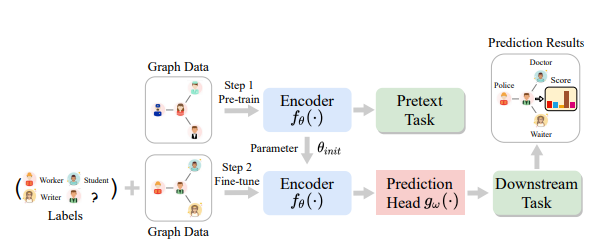
\includegraphics[width=.70\linewidth]{ssgnn1.png}
\end{figure}
\section{Joint learning}
If any specific pretext-task and downstream task is known, in such a situation, we can train the encoder with the prediction head. This strategy comes under multitask learning and jointly training the encoder and prediction head makes it joint learning. The below image can be a representation of this type of learning strategy.
\begin{figure}[h]
	\centering
	\hspace{21pt}
	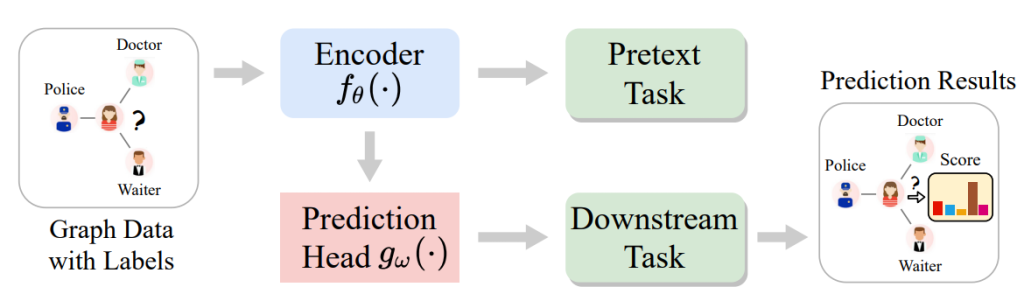
\includegraphics[width=.70\linewidth]{ssgnn2.png}
\end{figure}
\section{Unsupervised Representation Learning}
This strategy is pretty similar to the pretraining and fine-tuning strategy because the first step of the training is similar in both strategies. But here in the unsupervised representation learning strategy, we make the pre-trained parameters frozen so that the model can be trained on the frozen representation with downstream tasks only. The image below can be a representation of learning using this strategy.
\begin{figure}[h]
	\centering
	\hspace{21pt}
	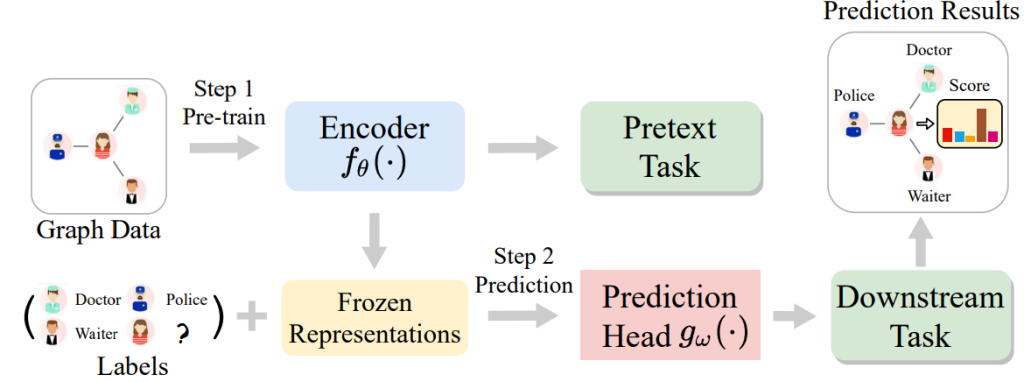
\includegraphics[width=.70\linewidth]{ssgnn3.png}
\end{figure}

Here in this section, we have seen what are three major strategies which can be followed to apply self-supervised learning on graph data. Considering the older work in this field, we can find there are specific categories of work performed using the graph data under the self-supervised learning settings. In the next section, we will discuss the different categories of old methods.

\chapter{Categorization of Self-Supervised Learning method for Graph Data}

Various works have been performed for self-supervised learning using graph data. By taking an overview from these works, we can say that methods under this field can be divided into three categories:

\section{Contrastive Learning}
We can find many works related to contrastive learning in the field of computer vision and natural language processing where in between some of the works are also there which represents the use of graph data in contrastive learning. By Generalizing them, we can find that the method works by generating multiple views of every instance through the data augmentation of the graph data. Furthermore, two views of the same instance can be considered as the positive pairs and two views from the different instance can be considered as the negative pair. After that the work of contrastive learning starts, which is to make the strong agreement between positive pairs and weak agreement between the negative pair.

For example, on a given graph we can apply different transformations to get multiple views, then a set of encoders can be applied on the multiple views to generate different representations of each view, where the contrastive learning will aim to maximize the mutual information of two views. Sum-up view of this method can be represented by the following image.

\begin{figure}[h]
	\centering
	\hspace{21pt}
	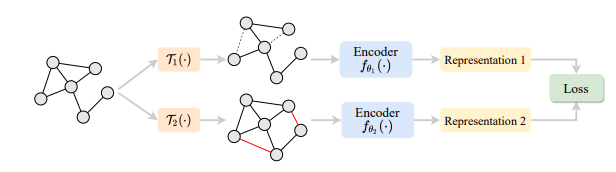
\includegraphics[width=.70\linewidth]{ssgnn4.png}
\end{figure}
\section{Generative learning}
The generative methods are based on the traditional generative models where embeddings that are holding rich information can be treated as natural self-supervision. In various studies we find that the prediction head works as a graph decoder; this decoder can also be used for graph reconstruction. A sum-up view of this method can be represented by the following image.
\begin{figure}[h]
	\centering
	\hspace{21pt}
	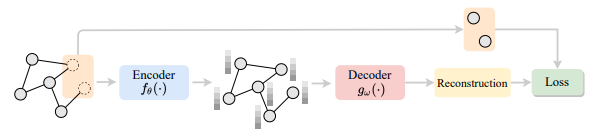
\includegraphics[width=.70\linewidth]{ssgnn5.png}
\end{figure}

The works related to generative methods focus on the information embedded in the graph, generally based on tasks such as reconstruction, which helps in exploiting the properties of graph data as self-supervision signals.

\section{Predictive Learning}
In many works, we can find out that they are focused on self-generative informative labels from the data as supervision. To obtain the labels on the data this method can follow the following ways:

\begin{itemize}
\item[1.] Node Property Prediction: Pre-calculation of properties can be used as self-supervised labels to utilize them for prediction.

\item[2.] Context-Based Prediction: Contextual information from the graph can be extracted to perform self-supervised learning. Information can be local or global.

\item[3.] Self Training: In this way, the predictive models can use the learned from pseudo-labels from clustering or random assignment.

\item[4.] Domain Knowledge Based Prediction: Subject matter experts or tools can be used in advance to analyze the graph data so that informative labels can be obtained on the graph.
\end{itemize}

\chapter{Related Works}
\section{Graph Neural Recommendation Models}
In recent years, the development of graph neural networks has provided a strong foundation and opportunity for developing graph-related hybrid recommendation tasks6,7. In particular, GCN8,9,10, a general formulation of GNNs, is a first-order approximation to spectral graph convolution and has driven many graph neural recommendation models, such as GCMC5, NGCF11, and LightGCN4. These GCN-based graph neural networks all adopted embedding propagation to iteratively aggregate neighborhood embeddings. By stacking the propagation layers, each node can access the embeddings of higher-order neighbors12, instead of only first-order neighbors as in the traditional methods [MF, NCF]113. Therefore GNN-based methods are the latest approaches in recommender systems with their advantages of handling structural and structural data.

\section{Self-Supervised Learning in Recommender Systems}\label{AA}
Self-supervised learning focuses on mining its supervised signals from large-scale unsupervised data using an auxiliary task (pretext). Then, it trains the model with such constructed supervised signs to learn valuable representations for downstream tasks. The mainstream self-supervised learning includes three main categories: generative, contrastive, and adversarial, all of which have a wide range of applications14. In visual representation learning, several self-supervised targets are introduced to guide visual feature learning using intrinsically relevant supervised signals15,16. In natural language processing, the model learns to predict the next word or sentence based on the sequence above17,18. In addition, self-supervised learning is also widely used in graph data learning19,20,21. For example, InfoGraph22 and DGI23 learn node representations based on mutual information between nodes and local structures.

Inspired by the results of self-supervised learning in graph learning, some recent studies24,25,26 have transposed it to the recommendation scenario. S3-Rec25 tried to use the principle of mutual information maximization to perform sequence recommendations. In addition, Wu et al.26 summarized all the stochastic enhancements on the graph and unified them into a general self-supervised graph learning framework for the recommendation.

In contrast to the above methods, our work is the first to consider both intra-node features and inter-node correlations generated through pre-training tasks. In power-law distributed data, these generative signals with the attention mechanism can motivate the model to consider both head and long-tail information to improve the recommendation performance.

\chapter{Conclusion}
In recent years, self-supervised learning has emerged as a promising approach to improve the performance of graph neural networks (GNNs) in various graph-related tasks. Self-supervised learning techniques aim to learn useful representations of the graph by predicting certain graph properties or performing certain tasks on the graph without relying on labeled data.

Self-supervised GNNs have shown great potential in various domains, including social network analysis, drug discovery, and traffic prediction. These models can learn meaningful representations of the graph that capture important structural information, leading to improved performance on downstream tasks.

Self-supervised learning also comes with its own set of challenges. For instance, designing effective self-supervised tasks that can capture meaningful graph properties can be difficult. Additionally, the performance of self-supervised GNNs can be highly dependent on the quality and diversity of the input data.

In conclusion, self-supervised GNNs have shown significant promise in advancing the state-of-the-art in graph-related tasks. As researchers continue to develop new and more effective self-supervised learning techniques, we can expect self-supervised GNNs to become an increasingly important tool in various applications.

\chapter{References}

\begin{itemize}
\item[[1]] Self-Supervised Learning of Graph Neural Networks: A Unified Review

https://ieeexplore.ieee.org/abstract/document/9764632

\item[[2]] SLAPS: Self-Supervision Improves Structure Learning for Graph Neural Networks

https://proceedings.neurips.cc/paper/2021/hash/bf499a12e998d178afd964adf64a60cb-Abstract.html

\item[[3]] From Canonical Correlation Analysis to Self-supervised Graph Neural Networks

https://proceedings.neurips.cc/paper/2021/hash/00ac8ed3b4327bdd4ebbebcb2ba10a00-Abstract.html

\item[[4]] Self-supervised Heterogeneous Graph Neural Network with Co-contrastive Learning

https://dl.acm.org/doi/abs/10.1145/3447548.3467415

\item[[5]] Self-supervised Graph Neural Networks without explicit negative sampling

https://arxiv.org/abs/2103.14958

\vspace{12pt}
\end{itemize}
\end{document}
